\section{Diskussion der Ergebnisse}

\subsection{Durchlassfilter}
Beim Aufzeichnen der Spannungskurven für verschiedene Ohmsche Wiederstände fiel auf, dass die Maxima im Vergleich zu denen der Theoriekurven viel zu klein waren. (siehe Abb. 5 \ref{plot:durchlass+R_ges-fit})
\paragraph{}Abb. \ref{plot:durchlass+R_ges-fit} zeigt die gleiche Messreihe, nur wurde hier zur Berechnung der Theoriekurve der Gesamtwiederstand des Stromkreises von 5.4 Ohm verwendet. Den größten Anteil an diesem Wert hatte die Spule.\\
Die geringen Abweichungen, die unter Berücksichtigung dieses Wiederstandes noch zu sehen sind, könnten unter anderem auf ungenauigkeiten der Messung mit dem "Sensor-Cassy" sowie auf ungenaue Kapazitäts- und Induktivitäts-Angaben zurückgeführt werden, fallen allerdings kaum ins Gewicht.
\subsection{Sperrfilter}
Genau so verhält es sich mit den aus dem Betrieb der Schaltung als Sperrfilter entstandenen Kurven. Nach Berücksichtigung des Ohmschen Wiederstandes der Spule ergeben sich nur noch minimale Abweichungen der Theorie zu den Messwerten, einzig die Resonanzfrequenz konnte nicht getroffen werden. Hier schien es uns am warscheinlichsten, dass der Wert der Induktivität der zweiten Spule mit 36 mH nicht korrekt war.
\begin{figure}
        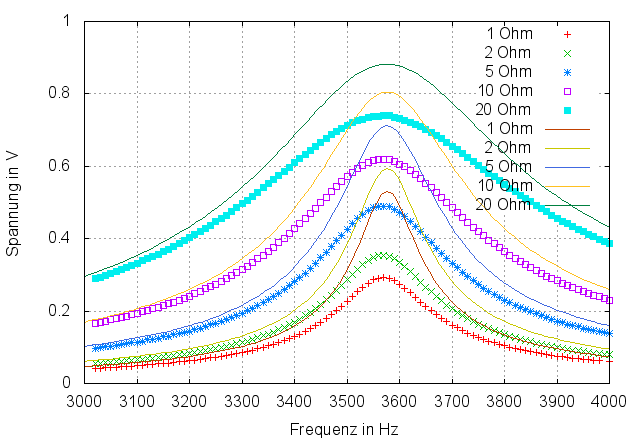
\includegraphics[width=.9\textwidth]{images/plot/durchlassfilter+theorie+R_ges.png}
\caption{Plot der Messdaten des Durchlassfilters (unter Vernachlässigung des Restlichen Wiederstandes)}
\label{plot:durchlass+R_ges}

	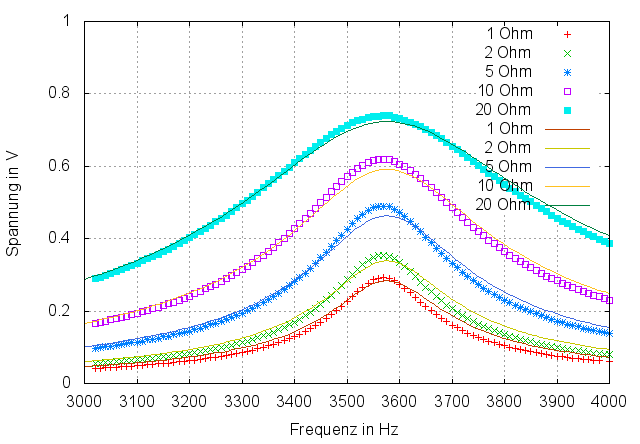
\includegraphics[width=.9\textwidth]{images/plot/durchlassfilter+theorie+R_ges-fit.png}
\caption{Plot der Messdaten des Durchlassfilters unter Berücksichtigung des gefitteten Gesamtwiederstandes}
\label{plot:durchlass+R_ges-fit}
\end{figure}
\begin{figure}
        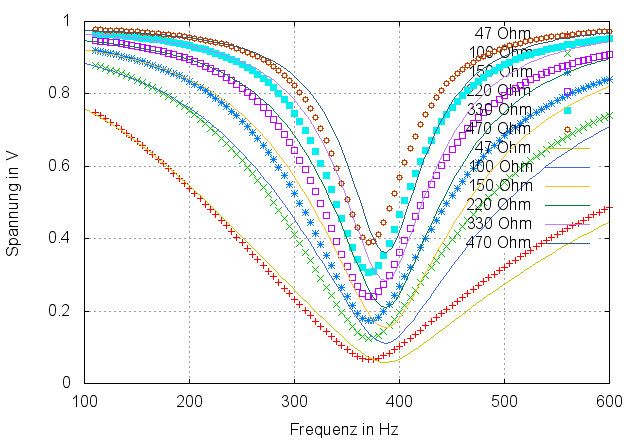
\includegraphics[width=.9\textwidth]{images/plot/sperrfilter+theorie+R_L.png}
\caption{Plot der Messdaten des Sperrfilters mit Theoriekurven}
\label{plot:sperr}
\end{figure}
